\lipsum[1]\cite{Desrat:2006}

\section{Uma seção qualquer}

\lipsum[2-3]

\begin{figure}
	\centering
	\psfrag{S}[][]{Fonte}
	\psfrag{2}[][]{$2$}
	\psfrag{3}[][]{$3$}
	\psfrag{D}[][]{Dreno}
	\psfrag{5}[][]{$5$}
	\psfrag{6}[][]{$6$}
	\psfrag{1mm}[][]{\unit{1}{\milli\metre}}
	\psfrag{V1}[][]{$V_H$}
	\psfrag{V}[][]{$V$}
	\psfrag{I0}[][]{$I = 0$}
	\psfrag{I}[][]{$I$}
	\psfrag{RA}[][]{\shortstack{Região de\\ interesse}}
	\psfrag{200}[l][l]{\unit{200}{\micro\metre}}
	\psfrag{500}[l][l]{\unit{500}{\micro\metre}}
	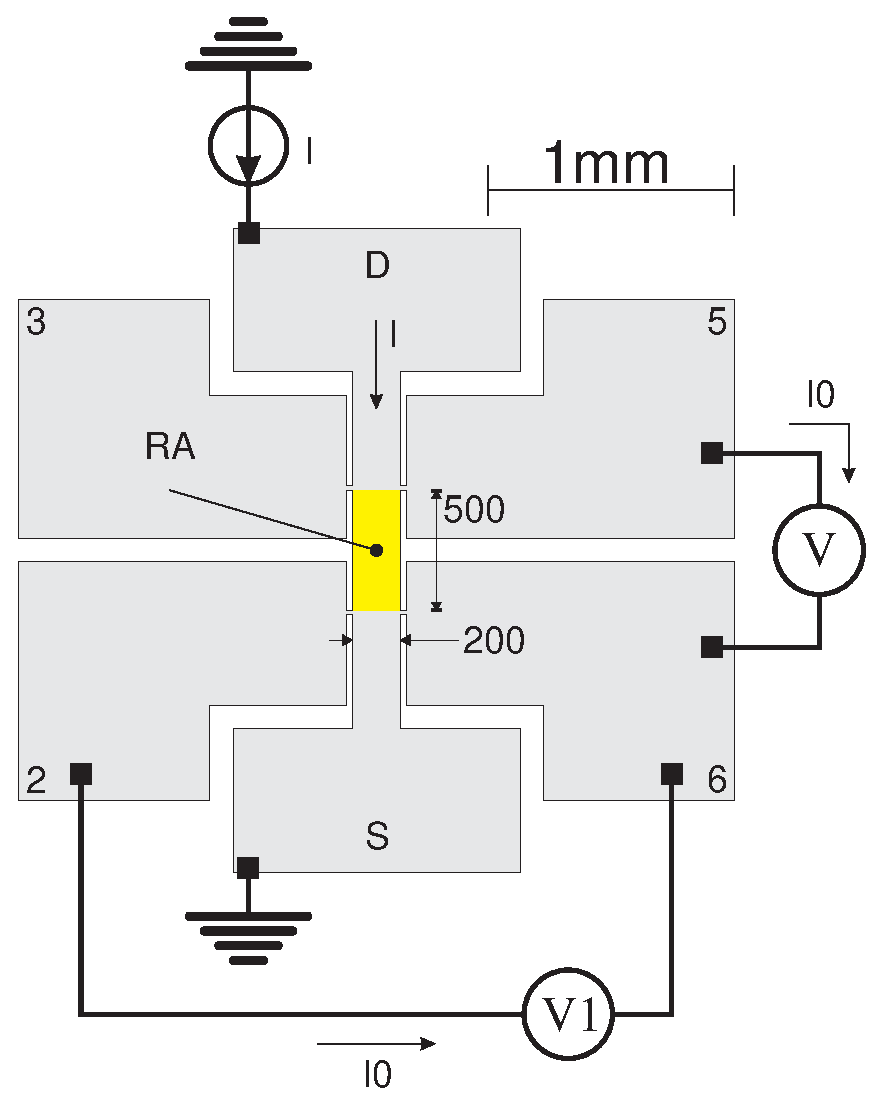
\includegraphics[height=0.4\textheight]{bH}
	\caption[Legenda curta]{o comando \cs{psfrag} (pacote \pkg{psfrag}) substitui os textos \emph{na figura EPS} por textos com a fonte deste documento. Mas isto só ocorre se a figura inserida aqui for EPS, ou seja, apenas se a compilação estiver produzindo um arquivo PostScript. Compare esta com a figura~\ref{fig:AB}, onde não efetuamos a substituição de texto.}
	\label{fig:if}
\end{figure}

\lipsum[4-5]

\section{Mais outra seção}

\lipsum[6]

Citando um livro: \cite{Eisberg:2000}

\lipsum[7-9]